\documentclass{beamer}

% Theme settings
\usetheme{Madrid} % Madrid theme provides a similar header and footer structure

% Color definitions (approximate based on the image)
\definecolor{darkblue}{RGB}{40,40,150} % For headers, footers, and boxes
\definecolor{lightblue}{RGB}{180,180,250} % For highlight within boxes
\usepackage[utf8]{inputenc}
\usepackage[T1]{fontenc}
\usepackage[backend=biber,style=numeric]{biblatex}
% Apply colors.sty
\setbeamercolor{palette primary}{bg=darkblue,fg=white}
\setbeamercolor{palette secondary}{bg=darkblue,fg=white}
\setbeamercolor{palette tertiary}{bg=darkblue,fg=white}
\setbeamercolor{palette quaternary}{bg=darkblue,fg=white}
\setbeamercolor{sidebar}{bg=darkblue,fg=white}
\setbeamercolor{frametitle}{bg=darkblue,fg=white}
\setbeamercolor{title}{bg=darkblue,fg=white}
\setbeamercolor{section in head/foot}{bg=darkblue,fg=white}
\setbeamercolor{subsection in head/foot}{bg=darkblue,fg=white}
\setbeamercolor{footline}{bg=darkblue,fg=white}

% For the boxes "Definition", "Theorem", "Example"
\setbeamercolor{block title}{bg=darkblue,fg=white}
\setbeamercolor{block body}{bg=lightblue,fg=black}

% Font settings (default Beamer fonts are often sans-serif, similar to the image)

\usepackage{lmodern} % A good sans-serif font often used with Beamer

% Custom logo (replace 'profmai_logo.png' with your actual logo file)
% Make sure the logo is in the same directory as your .tex file or provide the full path.
\usepackage{tikz}

\addbibresource{bibliography.bib}

\title{Architecture of DeepSeek-V3}
\author{Molnár Botond}
\date{\today} 


\begin{document}


\begin{frame}[noframenumbering]
    \titlepage
\end{frame}

\section{Transformer Models}

\begin{frame}
    \frametitle{Transformer Model Origins}
    Transformer models were first introduced in the Paper "Attention is all you need" in 2017, which arguably launched the artificial intelligence revolution. 
    It introduced the \textbf{self-attention} mechanism which enables the model to understand the whole context of the input without using convolution or sequence based RNNs. \cite{vaswani2017attention}
\end{frame}

\begin{frame}{Why not Convolution?}
    \begin{itemize}
        \item Convolution is excellent at capturing local patterns, but since they have a limited view on the whole context it falls short of capturing global context. \cite{CNNfield}
        \item The weights of CNNs are constant and learned during training, hence applying the same transformation across the same input. (In transformer models these weights come from the self-attention head $\rightarrow$ calculated dynamically)
    \end{itemize}
\end{frame}




\begin{frame}{Why not Recurrent Neural Networks (RNN)?}
    \begin{itemize}
        \item However, the problem of vanishing/exploding gradients has been solved by newer models (LSTM, GRU) they still struggle to maintain "attention". For example, when the model goes through the sequence it might "forget" the early parts of the message or might become insignificant. \cite{heycoachRNN}
        \item Its sequential processing nature prevents efficient parallelization (the $t$-th step depends on the $t-1$-th step), which makes it  time consuming to train the model. \cite{eitcaRNNchallenges}
        \item It has a  fixed sized hidden state (fixed size vector). As the sequence progresses, this vector must continuously update to summarize all relevant past information. For very long sequences, this leads to an information compression problem, where the hidden state cannot retain all the nuances of the entire history. \cite{ibmRNN}
    \end{itemize}
\end{frame}

\begin{frame}{Transformer Model Architecture}
    \begin{center}
        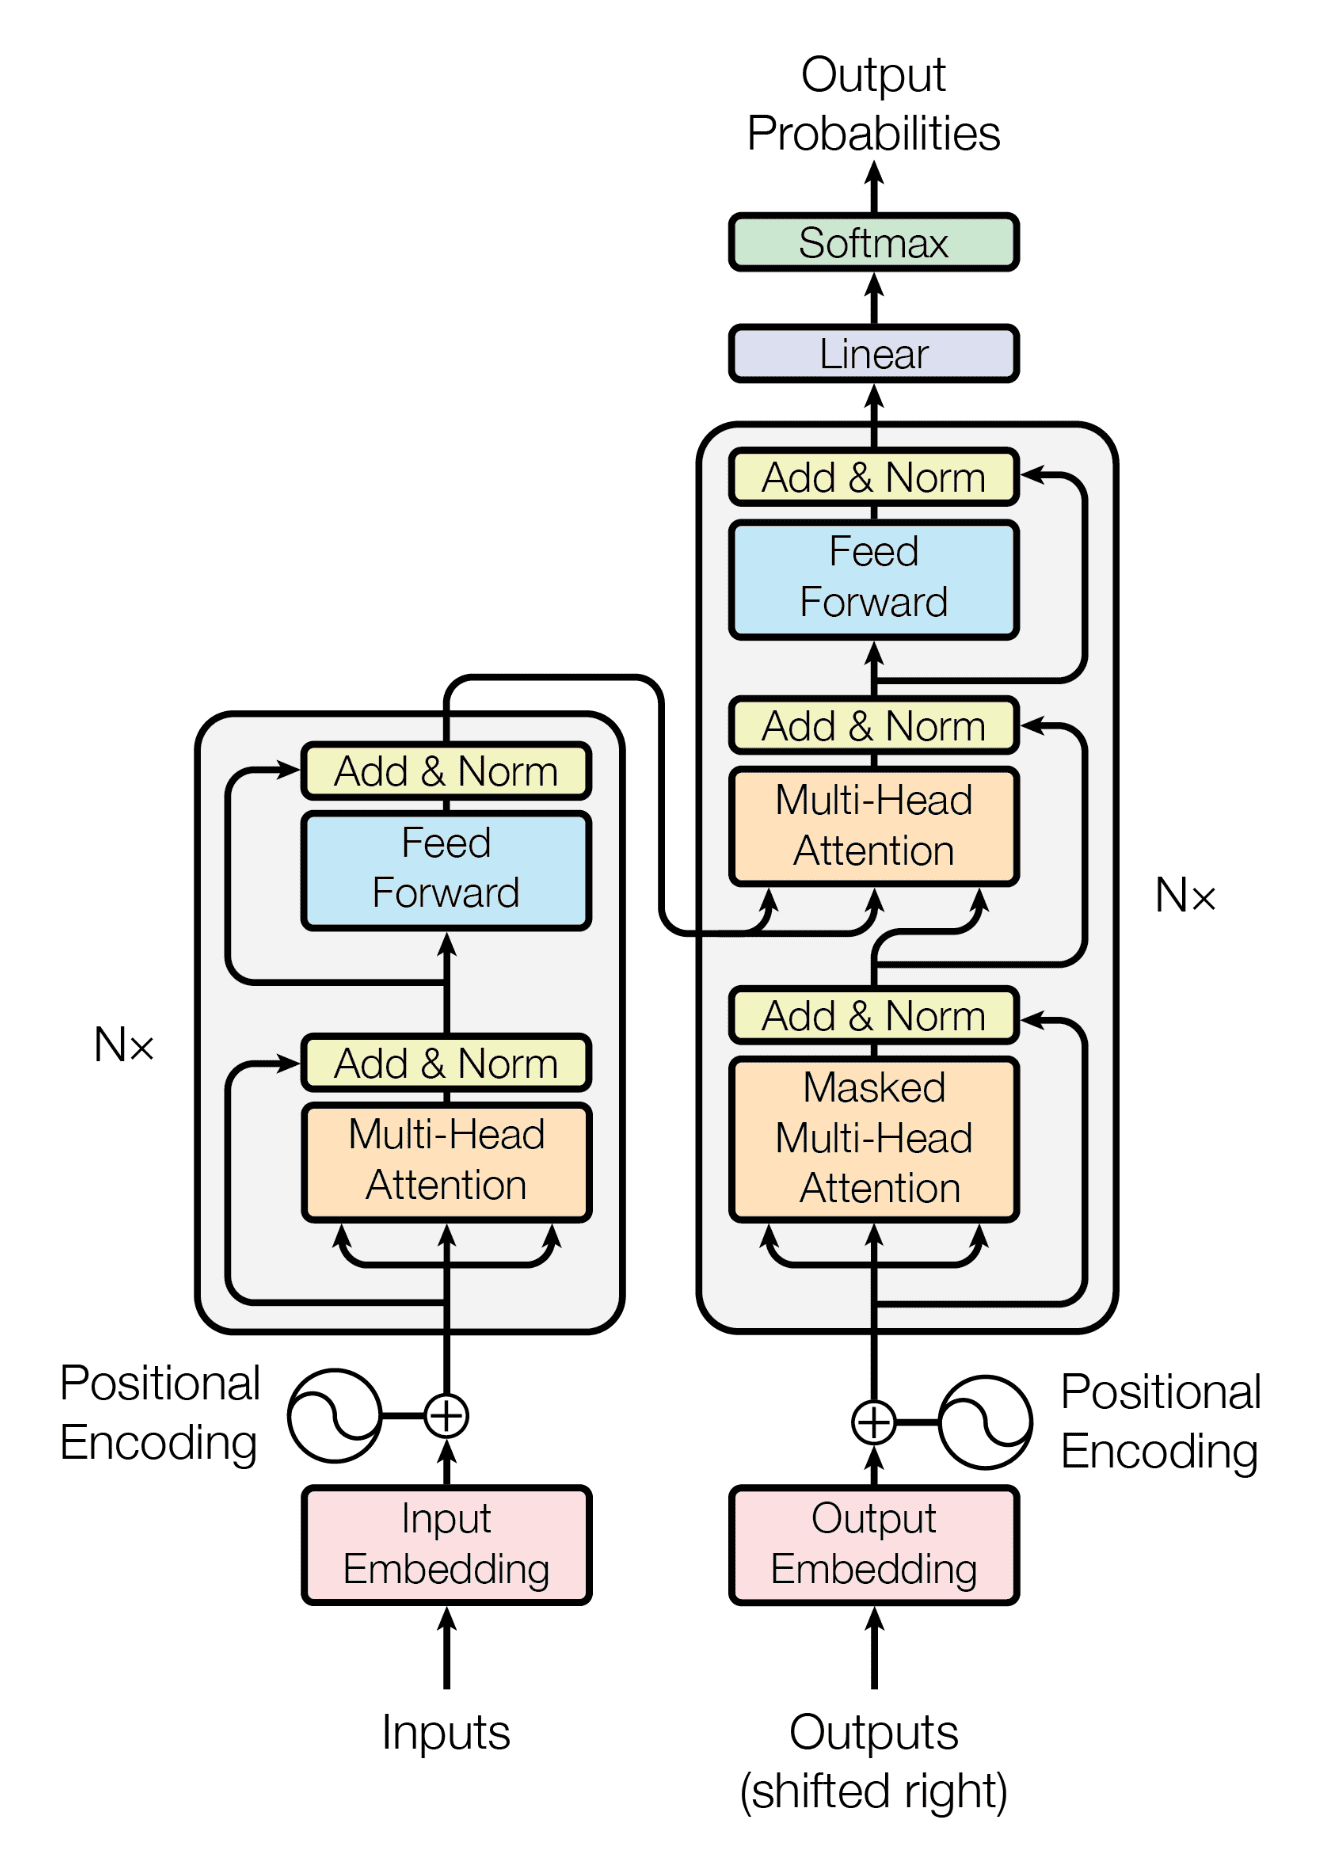
\includegraphics[width=0.4\textwidth]{transformer_model.png}
        \par
        \small Source:  \cite{vaswani2017attention}
    \end{center}
    
\end{frame}

\begin{frame}{Input Processing}
\begin{itemize}
    \item The input text must first be converted into numerical representation, usually using byte-pair encoding done on subword level.
    \item Then each token gets assigned a numerical ID.
\end{itemize}

\textbf{Example:} \\
\vspace{1em}
Raw text: \textit{The quick brown fox jumps.} \\
$\rightarrow$ ["The", "quick", "brown", "fox", "jump", "\#\#s", "."] (\#\# signals the continuation of a word) \\
$\rightarrow$ [101, 234, 567, 890, 123, 456, 789]
\end{frame}


\begin{frame}{Word Embedding}
\begin{itemize}
    \item \textbf{Learned Embeddings}: The transformer uses learned embeddings to convert the input tokens and output tokens to vectors of dimension $d_{model}$. It learns these representation during the training process.
    \item \textbf{Embedding Table}: $V \times d_{model}$ matrix, where each row represents a unique token in the vocabulary
    \item \textbf{Lookup Process}: After the token enters the embedding layer the model simply "looks up" the corresponding row in this embedding table. The entire row is the vector representation for that token.
\end{itemize}


\vspace{1em}
Output:
$$E \in \mathbb{R}^{n \times d_{model}}$$


$V$: vocabulary size \\ $d_{model}$: dimension of the model \\ $n$: number of tokens
    
\end{frame}

\begin{frame}{Position Encoding}
Since transformer models do not have recurrence or convolution, the order of words is not inherently captured, therefore positional encodings must be used. \cite{vaswani2017attention} uses sine and cosine functions to achieve this:

$$ PE_{(\text{pos},2i)} = \sin(\text{pos}/10000^{2i/d_{\text{model}}}) $$
$$ PE_{(\text{pos},2i+1)} = \cos(\text{pos}/10000^{2i/d_{\text{model}}}) $$

$$Input_{model} = E + EP \in \mathbb{R}^{n \times d_{model}}$$

\vspace{1em}
Where $pos$ is the position of the token and $i$ is the dimension.
    
\end{frame}

\section{Encoder Layer}

\begin{frame}{Encoder Attention Head}
    \begin{center}
        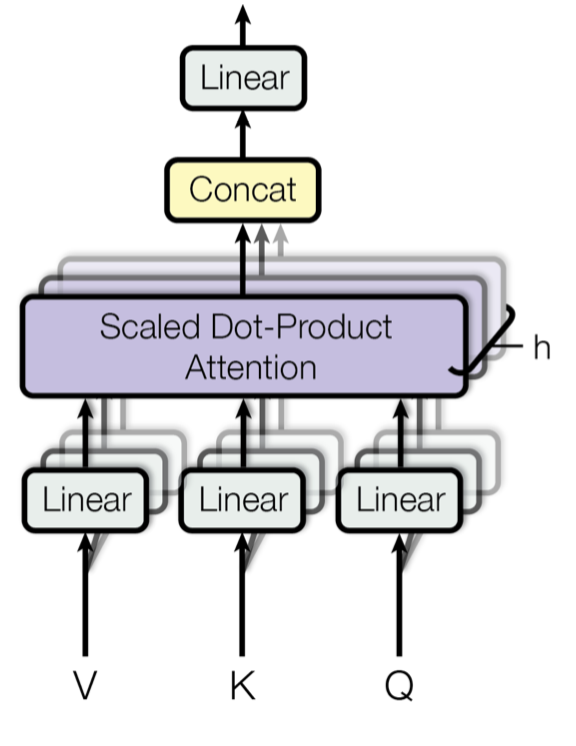
\includegraphics[width=0.4\textwidth]{multi-head-attention_l1A3G7a.png}
        \par
        \small Source:  \cite{vaswani2017attention}
    \end{center}
\end{frame}

\begin{frame}{Encoder Attention Head}

Each encoder attention head's input consists of the $Query$ ($Q$), $Key$ ($K$), $Value$ ($V$).
These values are linearly transformed from the embeddings using learned weights into lower dimensions:

$$Q_i = QW_i^Q$$
$$K_i = KW_i^K$$
$$V_i = VW_i^V$$

Where $Q_i$, $K_i$, $V_i$ $\in \mathbb{R}^{(d_{model}/h)}$, \\
$W_i^Q \in \mathbb{R}^{d_{model} \times d_k}$ \\
$W_i^K \in \mathbb{R}^{d_{model} \times d_k}$ \\
$W_i^V \in \mathbb{R}^{d_{model} \times d_v}$ \\
$h$ is the number of attention heads.  \\
$i$ is the index of the attention head. \cite{vaswani2017attention}
\end{frame}

\begin{frame}{Encoder Attention Head}
\begin{itemize}
    \item \textbf{Query (Q)}: Represents what each token attends to
    \item \textbf{Key (K)}: Represents what each token offers as context
    \item \textbf{Value (V)}: The actual content that gets aggregated
\end{itemize}
\end{frame}

\begin{frame}{Scaled Dot-Product Attention}
    $$ \text{Attention}(Q, K, V) = \text{softmax}\left(\frac{QK^T}{\sqrt{d_k}}\right)V $$

    Where \\ $Q \in \mathbb{R}^{n \times d_k}$, \\
    $K \in \mathbb{R}^{n \times d_k}$, \\
    $V \in \mathbb{R}^{n \times d_v}$. \\
    (In a transformer $d_k = d_v = d_{model}/h$ \cite{vaswani2017attention})

\end{frame}


\begin{frame}{Scaled Dot-Product Attention}
    \begin{itemize}
        \item $QK^T \in \mathbb{R}^{n \times n}$: Similarity between each \textit{Query} and \textit{Key} is computed. Result of the operation is often
        called the \textit{"attention scores"}. A large positive dot product indicates high similarity or 
        relevance between the query at position i and the key at position j. 
        This matrix essentially tells us, for each token in the sequence (represented by a query), how much it relates to every other token in the sequence (represented by keys).
        \item Scaling by $\sqrt{d_k} \left( \frac{QK^T}{\sqrt{d_k}} \right)$: he raw dot products can 
        become very large in magnitude, especially with larger $d_{model}$. 
        This can push the softmax function into regions where its gradients are extremely small (vanishing gradient).
        Dividing by $\sqrt{d_k}$ (the square root of the key dimension) normalizes these dot products, preventing them from becoming too large 
        and ensuring more stable gradients for the softmax.
    \end{itemize}
\end{frame}

\begin{frame}{Scaled Dot-Product Attention}
  \begin{itemize}
    \item Softmax function ($softmax(\cdot)$): The softmax function converts the scores into a probability distribution.
    Let $A_{ij} = \frac{(QK^T)_{ij}}{\sqrt{d_k}}$. Then, the softmax is applied row-wise: $\text{softmax}(A_i) = \frac{e^{A_{i,j}}}{\sum_{k=1}^n e^{A_{i,k}}}$ for each row $i$.
    Output of the $softmax(\cdot)$ is the \textit{"attention weight matrix"}: $W \in \mathbb{R}^{n \times n}$. 
    \item Multiplication with the \textit{Value (V)} matrix ($W \cdot V$): This multiplication effectively takes a weighted sum of the \textit{Value} vectors, 
    where the weights are given by the attention weight matrix $W$. This step aggregates the information from the relevant parts of the sequence into a single context-aware representation for each position.
    $$head_j = W \cdot V$$
    $$head_j \in \mathbb{R}^{n \times d_v}$$
    Where $j$ is the index of the attention head.
  \end{itemize}
\end{frame}


\begin{frame}{Concatenate Outputs From Attention Heads}

$$MultiHead(Q,K,V) = Concat(head_1, ..., head_h)W^O \in \mathbb{R}^{n \times d_{model}}$$

where $head_j = Attention(QW_i^Q, KW_i^K, VW_i^Q) \in \mathbb{R}^{n \times (h \cdot d_k)}$, \\ 
(since $h \cdot d_k = h \cdot (d_{model}/h) = d_{model}$) \\
$W^O \in \mathbb{R}^{hd_v \times d_{model}}$ : Learned linear projection\\
$n$: sequence length

\end{frame}

\begin{frame}{Add and Norm Layer}
  The output of the Multi-Head Attention is added to its input ($Z^{(l-1)}$) and then layer normalized.

  $$ Z_{attention\_normalized} = LayerNorm(Z^{(l-1)} + MultiHead(\cdot)) \in \mathbb{R}^{n \times d_{model}} $$
\end{frame}


\begin{frame}{Layer Normalization}
  For an input vector $x$ (a row in the matrix), it normalizes over the features \cite{ba2016layer}:
  $$ \mu = \frac{1}{d_{\text{model}}} \sum_{i=1}^{d_{\text{model}}} x_i \text{ (mean)} $$
  $$ \sigma^2 = \frac{1}{d_{\text{model}}} \sum_{i=1}^{d_{\text{model}}} (x_i - \mu)^2 \text{ (variance)} $$
  $$ \text{LayerNorm}(x_i) = \gamma \frac{x_i - \mu}{\sqrt{\sigma^2 + \epsilon}} + \beta $$
   $\gamma$ and $\beta$ are learned scaling and shifting parameters, respectively. \\
   $\epsilon$ is a small constant for numerical stability (to prevent division by zero).
\end{frame}


\begin{frame}{Position-wise Feed-Forward Network}
  This sub-layer is applied to each position independently and identically. 
  It consists of two linear transformations with a ReLU activation in between. \\
  Let the input be $Z_{attention\_normalized}$

  $$ \text{FFN}(Z_{attention\_normalized}) = \max(0, xW_1 + b_1)W_2 + b_2 $$

  \begin{itemize}
    \item $ W_1 \in \mathbb{R}^{d_{\text{model}} \times d_{\text{ff}}} \text{ (e.g., } 512 \times 2048) $
    \item $b_1 \in \mathbb{R}^{d_{ff}}$
    \item $max(0, \cdot)$ is the ReLU activation function
    \item $W_2 \in \mathbb{R}^{d_{\text{ff}} \times d_{\text{model}}} \text{ (e.g., } 2048 \times 512)$
    \item $b_2 \in \mathbb{R}^{d_{\text{model}}}$
    \item Let the output be $FFN_{output} \in \mathbb{R}^{n \times d_{model}}$ $\rightarrow$ This will be passed to another \textbf{Add and Norm} sublayer
    whose output will be passed to the next encoder layer. 
  \end{itemize}
\end{frame}


\begin{frame}{Final Encoder Output}
  After passing through all $N$ encoder layers, the output of the last layer ($Z^{(N)}$) is a sequence of $n$ vectors, each of dimension $d_{\text{model}}$. These vectors are dense, contextualized representations of the input sequence. This final output of the 
  encoder stack is then passed to the decoder's "encoder-decoder attention" mechanism. \cite{vaswani2017attention}
\end{frame}

\section{Decoder Layers}

\begin{frame}{Decoder Layer}
  The decoder in the Transformer model is responsible for generating the output sequence one token at a time, incorporating context from both the input sequence (via the encoder)
  and the tokens it has already generated. It operates in an auto-regressive fashion.
  
  Each of the N identical layers within the decoder stack is composed of three 
  main sub-layers, each followed by a residual connection and layer normalization.

  The main difference to the encoder layer is a new sub-layer, the multi-head self-attention.
\end{frame}

\begin{frame}{Decoder Layer}
  \begin{itemize}
    \item Let the input be $Y^{(l-1)}$ for the current decoder layer $l$. (output from the previous decoder layer 
    or the combined embedding and positional encoding of the partial output sequence for the first layer)
    \item The encoder's final output $ Z_{\text{enc}}^{(N)} $ , serves as the memory for the encoder-decoder attention.
  \end{itemize}

  \begin{itemize}
    \item $Y^{(l-1)} \in \mathbb{R}^{m \times d_{model}}$ 
    \item $m$: current length of the partial output sequence being generated
    \item $ Z_{\text{enc}}^{(N)} \in \mathbb{R}^{n \times d_{\text{model}}} $
  \end{itemize}
  
\end{frame}

\begin{frame}{Masked Multi-Head Self-Attention Sub-layer}
  \textbf{1. Input Projections for Q, K, V:}
  \begin{itemize}
    \item The input to this sub-layer is $Y^{(l-1)}$.
    \item For each of the $h$ attention heads ($j = 1, \dots, h$), $Y^{(l-1)}$ is linearly projected into Query ($Q_j$), Key ($K_j$), and Value ($V_j$) matrices using learned weight matrices $W^Q_j, W^K_j, W^V_j \in \mathbb{R}^{d_{\text{model}} \times d_k}$ (where $d_k = d_v = d_{\text{model}}/h$).
    \item $ Q_j = Y^{(l-1)}W^Q_j $
    \item $ K_j = Y^{(l-1)}W^K_j $
    \item $ V_j = Y^{(l-1)}W^V_j $
    \item $Q_j, K_j, V_j \in \mathbb{R}^{m \times d_k}$.
  \end{itemize}
\end{frame}

\begin{frame}{Masked Attention}
  \textbf{2. Masked Scaled Dot-Product Attention:}
  \begin{itemize}
      \item The core attention calculation is performed:
      $$ \text{head}_j = \text{softmax}\left(\frac{Q_j K_j^T + \text{Mask}}{\sqrt{d_k}}\right)V_j $$
      \item \textbf{The crucial difference here is the "Mask."} This is a look-ahead mask (upper triangular matrix of negative infinities) that is applied to the attention scores before the softmax function.
      \item It prevents each position in the decoder from attending to subsequent positions. When predicting the $i$-th token, the mask ensures that the calculation for $\text{head}_j$ only considers information from tokens at positions $1, \dots, i-1$. This is essential for maintaining the 
      auto-regressive property of the decoder, ensuring that predictions for future tokens do not influence current token generation.
      \item Everithing else works the same as in the encoder layers.
      \item Output: $\text{head}_j \in \mathbb{R}^{m \times d_k}$.
      \item $Mask \in \mathbb{R}^{m \times m}$
  \end{itemize}
\end{frame}


\begin{frame}{}
  
\end{frame}

\begin{frame}[allowframebreaks]
    \frametitle{References}
    \printbibliography
\end{frame}

\end{document}